\documentclass[dvisvgm,tikz,12pt]{standalone}
\usepackage{amsmath}
\usepackage{tikz}

\begin{document}
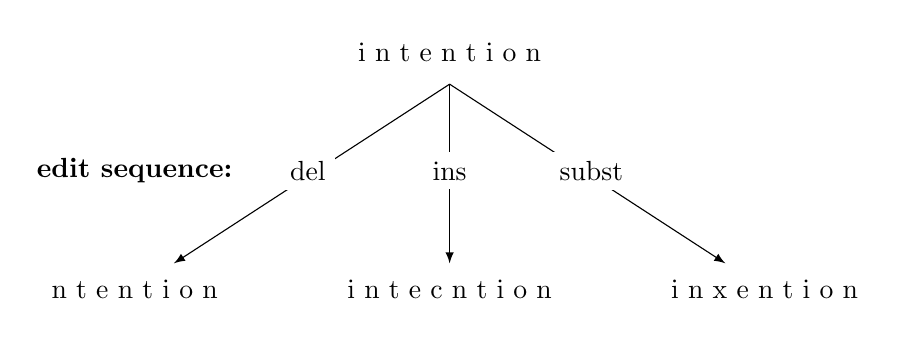
\begin{tikzpicture}
  \node[inner sep=0.2cm] (n1) at (0,0) {i n t e n t i o n};

  \node[inner sep=0.2cm] (n2) at (-4,-3) {n t e n t i o n};
  \node[inner sep=0.2cm] (n3) at (0,-3) {i n t e c n t i o n};
  \node[inner sep=0.2cm] (n4) at (4,-3) {i n x e n t i o n};

  \draw[-latex] (0,-0.4cm) -- (n2);
  \draw[-latex] (0,-0.4cm) -- (n3);
  \draw[-latex] (0,-0.4cm) -- (n4);

  \node[fill=white] at (-4,-1.5) {\textbf{edit sequence:}};
  \node[fill=white] at (-1.8,-1.5) {del};
  \node[fill=white] at (-0,-1.5) {ins};
  \node[fill=white] at (1.8,-1.5) {subst};
\end{tikzpicture}
\end{document}
